%% generato automaticamente da tools/build_tex.py --- non modificare
\chapter{Cinque modi di fabbricare $\pi$}
\label{cap:pigreco}
\quaderno{pigreco.dfw}{27 Aug 2010}{26}

Agosto 2010, lo stesso giorno di \dfw{numeri primi.dfw}. Ventisei espressioni divise in cinque episodi indipendenti, accomunati da un obiettivo: costruire $\pi$ a partire da oggetti in cui $\pi$ non sembra esserci. Il quarto episodio contiene un'identità esatta, che si riduce a due formule da manuale.

\section{Un operatore differenziale applicato due volte}

Si parte da una funzione di due variabili e le si applica l'operatore $D=\partial_x+\partial_y$, cioè la derivata direzionale lungo la bisettrice. Il quaderno calcola le due derivate parziali, le somma, e poi ripete l'operazione sul risultato.

\begin{espr}{1}{User}{}
\[
\frac{1}{\pi}\, \left(y - x\right)\, \left(x + \frac{1}{y}\right)
\]
\end{espr}
La funzione di partenza, con $\pi$ presente solo come fattore costante.

\begin{espr}{2}{Dif(\#1,x)}{}
\[
\frac{\mathrm{d}}{\mathrm{d}x}\!\left[\frac{1}{\pi}\, \left(y - x\right)\, \left(x + \frac{1}{y}\right)\right]
\]
\end{espr}
Si chiede la derivata rispetto a $x$.

\begin{espr}{3}{Simp(Dif(\#1,x))}{}
\[
-\frac{2\, x\, y - y^{2} + 1}{\pi\, y}
\]
\end{espr}
Il risultato, riordinato da Derive.

\begin{espr}{4}{Dif(\#1,y)}{}
\[
\frac{\mathrm{d}}{\mathrm{d}y}\!\left[\frac{1}{\pi}\, \left(y - x\right)\, \left(x + \frac{1}{y}\right)\right]
\]
\end{espr}
Ora rispetto a $y$.

\begin{espr}{5}{Simp(Dif(\#1,y))}{}
\[
\frac{x\, \left(y^{2} + 1\right)}{\pi\, y^{2}}
\]
\end{espr}
Il risultato.

\begin{espr}{6}{User}{}
\[
\frac{x\, \left(y^{2} + 1\right)}{\pi\, y^{2}} + -\frac{2\, x\, y - y^{2} + 1}{\pi\, y}
\]
\end{espr}
La somma delle due derivate parziali: è la derivata direzionale lungo la bisettrice.

\begin{espr}{7}{Simp(\#6)}{}
\[
\frac{\left(1 - y^{2}\right)\, \left(x - y\right)}{\pi\, y^{2}}
\]
\end{espr}
Semplificata. Il fattore $(x-y)$ è sopravvissuto alla derivazione.

\begin{espr}{8}{Dif(\#7,x)}{}
\[
\frac{\mathrm{d}}{\mathrm{d}x}\!\left[\frac{\left(1 - y^{2}\right)\, \left(x - y\right)}{\pi\, y^{2}}\right]
\]
\end{espr}
Si ricomincia: derivata rispetto a $x$ del risultato.

\begin{espr}{9}{Simp(Dif(\#7,x))}{}
\[
\frac{1 - y^{2}}{\pi\, y^{2}}
\]
\end{espr}
Il risultato non dipende più da $x$.

\begin{espr}{10}{Dif(\#7,y)}{}
\[
\frac{\mathrm{d}}{\mathrm{d}y}\!\left[\frac{\left(1 - y^{2}\right)\, \left(x - y\right)}{\pi\, y^{2}}\right]
\]
\end{espr}
Derivata rispetto a $y$.

\begin{espr}{11}{Simp(Dif(\#7,y))}{}
\[
\frac{y\, \left(y^{2} + 1\right) - 2\, x}{\pi\, y^{3}}
\]
\end{espr}
Il risultato.

\begin{espr}{12}{User}{}
\[
\frac{1 - y^{2}}{\pi\, y^{2}} + \frac{y\, \left(y^{2} + 1\right) - 2\, x}{\pi\, y^{3}}
\]
\end{espr}
La loro somma: la seconda applicazione dell'operatore.

\begin{espr}{13}{Simp(\#12)}{}
\[
\frac{2\, \left(y - x\right)}{\pi\, y^{3}}
\]
\end{espr}
Semplificata. Il fattore $(y-x)$ è ancora lì, e la potenza di $y$ al denominatore è salita a tre.


Il risultato dei due passaggi è che il fattore $(x-y)$ sopravvive a entrambe le applicazioni dell'operatore, mentre la dipendenza da $y$ si semplifica progressivamente: da $(1-y^2)/y^2$ si passa a $2/y^3$. La funzione di partenza è costruita in modo che $\pi$ compaia solo come costante moltiplicativa, e infatti attraversa indenne tutte le derivazioni. Sulla retta $y=1$ la derivata prima si annulla identicamente, e la funzione vi si riduce a $(1-x^2)/\pi$.

\section{Due prodotti che diventano fattoriali}

Un intermezzo di combinatoria. Due prodotti finiti con estremi legati alla variabile, e le forme chiuse che Derive ne ricava.

\begin{espr}{14}{User}{}
\[
\prod_{n=0}^{x} \left(x + n\right)
\]
\end{espr}
Un prodotto di $x+1$ fattori consecutivi a partire da $x$.

\begin{espr}{15}{Simp(\#14)}{}
\[
\frac{\left(2\, x\right)!}{\left(x - 1\right)!}
\]
\end{espr}
La sua forma chiusa: rapporto di due fattoriali.

\begin{espr}{16}{User}{}
\[
\prod_{n=0}^{x - 1} \left(x - n\right)
\]
\end{espr}
Il prodotto discendente da $x$ a $1$.

\begin{espr}{17}{Simp(User)}{}
\[
x!\, \cos^{2}\!\left(\pi\, x\right)
\]
\end{espr}
Derive scrive $x!\cos^2(\pi x)$: il fattore trigonometrico vale $1$ sugli interi, dove la formula è valida, e si annulla sui semi-interi.


Il secondo risultato merita attenzione. Il prodotto $x(x-1)\cdots1$ vale $x!$ per $x$ intero, ma l'espressione ha senso anche fuori dagli interi, e Derive restituisce $x!\cos^2(\pi x)$. Il fattore $\cos^2(\pi x)$ vale $1$ su tutti gli interi e si annulla sui semi-interi: è il modo del programma di dire che la forma chiusa è valida sugli interi e non altrove. È un'informazione, non un errore di semplificazione.

\section{$\pi$ da un fattoriale}

Tre righe, il modo più corto del quaderno per ottenere $\pi$.

\begin{espr}{18}{User}{}
\[
\left(\frac{1}{2}\right)!
\]
\end{espr}
Il fattoriale di un mezzo, cioè $\Gamma(3/2)$.

\begin{espr}{19}{Simp(\#18)}{}
\[
\frac{\sqrt{\pi}}{2}
\]
\end{espr}
Che vale $\sqrt{\pi}/2$.

\begin{espr}{20}{User}{}
\[
4\, \left(\frac{1}{2}\right)!^{2}
\]
\end{espr}
Si quadra e si moltiplica per quattro.

\begin{espr}{21}{Simp(\#20)}{}
\[
\pi
\]
\end{espr}
Il risultato è $\pi$ esatto.


Il fattoriale di un mezzo è $\Gamma(3/2)=\sqrt{\pi}/2$, e quadrando e moltiplicando per quattro si ottiene $\pi$ esatto. È l'unico posto in tutta la raccolta in cui la funzione Gamma compare in modo essenziale, e vi compare senza essere nominata.

\section{L'identità del rapporto}

Questo è il risultato principale del quaderno: un rapporto fra funzioni trigonometriche e arcotangenti che vale $\pi$ per ogni $x$ reale non nullo, cambiando segno con $x$.

\begin{espr}{22}{User}{}
\begin{align*}
& \frac{\left(\cos\!\left(2\, x\right) - \cos\!\left(\frac{2}{x}\right)\right)\, \left(\arctan\!\left(x\right) + \arctan\!\left(\frac{1}{x}\right)\right)}{\cos^{2}\!\left(x\right) - \cos^{2}\!\left(\frac{1}{x}\right)} \\
=\;& \operatorname{sgn}\!\left(x\right)\, \pi
\end{align*}
\end{espr}
L'identità centrale del quaderno. Vale per ogni $x\neq0$ in cui il denominatore non si annulla.

\begin{espr}{23}{User}{}
\begin{align*}
& \frac{\left(\sum_{n=0}^{\infty} \frac{\left(2\, x\right)^{2\, n} - \left(\frac{2}{x}\right)^{2\, n}}{\left(2\, n\right)!}\right)\, \sum_{n=0}^{\infty} \frac{\left(-1\right)^{n}}{\left(2\, n + 1\right)!}\, \left(x^{2\, n + 1} + x^{-2\, n - 1}\right)}{\left(\sum_{n=0}^{\infty} \frac{x^{2\, n}}{\left(2\, n\right)!}\right)^{2} + \left(\sum_{n=0}^{\infty} \frac{x^{-2\, n}}{\left(2\, n\right)!}\right)^{2}} \\
=\;& \operatorname{sgn}\!\left(x\right)\, \pi
\end{align*}
\end{espr}
La stessa identità con tutte le funzioni sostituite dai loro sviluppi in serie: una verifica della robustezza del risultato.

\begin{figure}[htbp]
  \centering
  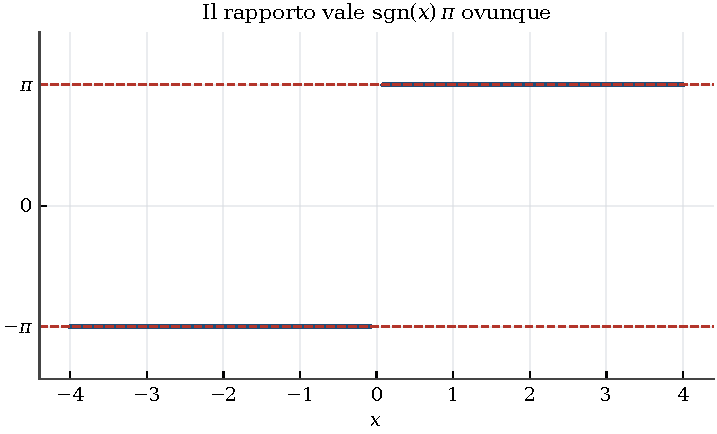
\includegraphics[width=0.86\linewidth]{../figures/pigreco_identita.pdf}
  \caption{Verifica numerica dell'identità $\#22$: il rapporto vale $\pi$ per $x>0$ e $-\pi$ per $x<0$, con le sole interruzioni nei punti in cui il denominatore si annulla.}
  \label{fig:pigreco_identita}
\end{figure}

L'identità è esatta e si dimostra in due mosse. La formula di duplicazione $\cos 2\theta=2\cos^2\theta-1$ trasforma il numeratore: $\cos 2x-\cos\tfrac2x=2\left(\cos^2 x-\cos^2\tfrac1x\right)$, e il rapporto con il denominatore vale dunque esattamente $2$, per ogni $x$ per cui il denominatore non si annulla. Resta il secondo fattore, $\arctan x+\arctan\tfrac1x$, che vale $\pi/2$ per $x>0$ e $-\pi/2$ per $x<0$: è l'identità classica dell'arcotangente del reciproco. Il prodotto è $2\cdot\mathrm{sgn}(x)\tfrac{\pi}{2}=\mathrm{sgn}(x)\,\pi$.

Detto altrimenti: il primo fattore è una costante travestita da funzione, il secondo è un gradino travestito da somma di arcotangenti, e il prodotto è un gradino di altezza $2\pi$. La riga $\#23$ riscrive la stessa cosa con gli sviluppi in serie di tutte le funzioni coinvolte, presumibilmente per verificare che l'identità non dipenda da proprietà nascoste delle funzioni chiuse.

\section{$\pi$ ed $\mathrm{e}$ come estremi di una stessa funzione}

L'ultimo episodio è il più breve.

\begin{espr}{24}{User}{}
\[
\left(\pi^{x} + \mathrm{e}^{x}\right)^{\frac{1}{x}}
\]
\end{espr}
La media di potenza di ordine $x$ fra $\pi$ ed $\mathrm{e}$.

\begin{espr}{25}{User}{\verificata}
\[
\lim_{x \to +\infty} \left(\pi^{x} + \mathrm{e}^{x}\right)^{\frac{1}{x}} = \pi
\]
\end{espr}
Per $x\to+\infty$ prevale la base maggiore.

\begin{espr}{26}{User}{\verificata}
\[
\lim_{x \to -\infty} \left(\pi^{x} + \mathrm{e}^{x}\right)^{\frac{1}{x}} = \mathrm{e}
\]
\end{espr}
Per $x\to-\infty$ prevale la minore. Una funzione, due costanti.


La funzione $\left(\pi^x+\mathrm{e}^x\right)^{1/x}$ è la media di potenza di ordine $x$ dei due numeri. Per $x\to+\infty$ il termine con la base maggiore domina e la media tende al massimo, cioè $\pi$; per $x\to-\infty$ domina il termine con la base minore e si ottiene $\mathrm{e}$. Una sola espressione contiene entrambe le costanti, ciascuna come limite da una parte. È lo stesso meccanismo per cui la norma $\ell^p$ di un vettore tende al massimo delle componenti quando $p$ diverge.

\section*{In sintesi}
\addcontentsline{toc}{section}{In sintesi}

Il quaderno raccoglie cinque strade indipendenti verso lo stesso numero: una derivazione ripetuta che lo lascia intatto, un prodotto che lo fa comparire in un fattore correttivo, un fattoriale semi-intero che lo produce esattamente, un rapporto trigonometrico che vale $\pi$ ovunque, e una media di potenze che lo raggiunge all'infinito. Solo la quarta è un'identità nel senso stretto — ed è anche l'unica che si dimostra in due righe.

